\begin{comment}
							

\end{comment}

\section{Introduction}
Predicting the next item of a sequence over a finite alphabet has various approaches where some of them contain a relatively extensive literature. The applications which are covered by these various prediction approaches vary and different challenges are addressed for each one. \emph{Lossless} approach is a new approach  recently introduced by \citeauthor{gueniche_fournier-viger_tseng_2013} \citeyear{gueniche_fournier-viger_tseng_2013}. Since it is a new approach, it is interesting to study it offering more solutions.
\section{Problem Definition}
Let a finite set of items (symbols) \(\Sigma = \{e_1, e_2,\ldots,e_\sigma\}\) be called \emph{alphabet}, then a \emph{sequence} \(S\) is a list of ordered items \(S=\langle i_1,i_2,\ldots,i_k\rangle\) where \(i_m \in \Sigma\ for\ 1\leq m \leq k\). A multiset of sequences \(D = \langle S_1, S_2,\ldots,S_l\rangle\) also called \emph{dataset} is constituted by sequences that created under a similar way. Given a dataset, a prediction algorithm is \emph{trained} on this dataset.  Once the prediction algorithm is trained, it will repeatedly accept a \emph{context} which is another sequence of symbols, and outputs a \emph{prediction}. The context is obtained from an unknown \emph{query sequence} which does not belong to the dataset but shares common characteristics with the dataset.  Loosely speaking, the context is derived from a part of the query sequence, and the prediction is about what comes \emph{after} the context in the query.

\section{Lossless}
Lossless sequence prediction is a relatively new approach and therefore appears to have quite a few challenges that someone that studies it has to cope with. It is clear that due to the fact that a whole dataset is utilised, a lossless approach achieves a higher space utilisation over a lossy approach. This fact leads to two results; firstly, it is somewhat intensive for an algorithm to go through all the data and extract the appropriate information needed for predictions, and secondly, keeping all the relative data \emph{in memory}, through the corresponding data structures, appears to be a considerably hard challenge because the represented structure's space utilisation often reaches an order of magnitude of the initial gathered data. As a result, a lossless sequence prediction approach needs sophisticated tools to search for patterns and sequences in \emph{Big Data} when simultaneously the aforementioned challenges are coped.
\par On contrary, a \emph{lossy} approach can be less memory hungry by representing the given information of a dataset through models (like \emph{dependency graphs}). This leads to implementation that sometimes utilises less space and can be potentially faster. However, a lossy approach lacks accuracy especially in hard cases when information in a dataset is not repeating as other parts of informations or a repetition is either generalised or ignored by a model having a partly loss of information that is not reversible. Often such hard cases lead to more complex models that along with Big data is hard to make algorithms that produce predictions with efficiency and performance.
\section{Motivation}
\todo{refer briefly to some SPICE results}
\section{CPT Predictor and its Data Structures}\label{CPT}
CPT and CPT+ (\textbf{C}ompact \textbf{P}rediction \textbf{T}ree) introduced by \citeauthor{gueniche_fournier-viger_tseng_2013} \citeyear{gueniche_fournier-viger_tseng_2013} and later improved by \citeauthor{gueniche_fournier-viger_raman_tseng_2015} \citeyear{gueniche_fournier-viger_raman_tseng_2015}, is currently the only implementation in lossless sequence prediction. It is constituted by a Trie (\emph{Prediction Tree PT}), an Array of bit-vectors (\emph{Inverted Index II}) and an array of pointers to the last items of sequences inserted to the prediction tree (\emph{Look-up Table LT}). As a lossless approach, CPT utilises the whole dataset provided for building its structures. Each sequence from the dataset is inserted to the Prediction Tree and a pointer to the last item of the sequence is added to the Look-up Table. The Inverted Index has the role of finding which sequence contains which alphabet's items by simply executing a bitwise AND operation. Every bit-vector has the same length with the total number of the dataset's sequences while it notes, using 1/0, whether an alphabet item appears in the sequence or not \ref{fig:CPT-structure}.
\par CPT can retrieve any searching sequence with specific alphabet items by using the inverted index along with a combination of the two other structures. A bitwise AND shows which sequences contain some given alphabet items and then these sequences can be located by using the Look-up Table which points to the end of each corresponding sequence. Having retrieved a requested sequence and along with the query sequence, a \emph{consequent} can be resulted as a part of the retrieved sequence. The consequent simply constitutes the sequence containing the remaining items after every item of the query (query on this case is used as a set) has been removed from the retrieved sequence. For example, if the sequence \(S_1=\langle a, b, x, z, c, d, e\rangle\) was retrieved from the prediction tree and the query sequence is \(S_q=\langle a, b, a, c\rangle\) then the consequent will be \(S_c=\langle d, e\rangle\). The produced consequent is then used by a \emph{prediction task} (see Appendix \ref{App:predtask}) in order for a prediction to get calculated.

\begin{figure}[h]
    \centering
    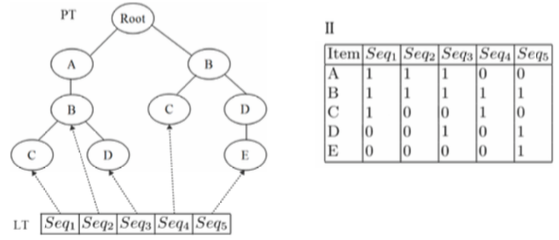
\includegraphics[width=0.75\textwidth]{CPT-structure}
    \caption{A Prediction Tree (PT), Inverted Index (II) and Lookup Table (LT)}
    \label{fig:CPT-structure}
\end{figure}

In Figure \ref{fig:CPT-structure} it is shown an example of CPT during multiple sequence insertions.

\subsection{Strengths \& Weaknesses}

CPT (as a lossless approach) utilises all the available sequences in a tree where they are accessible through the II and the LT easily and fast by a bitwise AND for each sequence. Therefore, making predictions can be potentially fast and accurate as described in \citep{gueniche_fournier-viger_tseng_2013} and \citep{gueniche_fournier-viger_raman_tseng_2015}. Locating similar sequences can be a relatively easy task that makes CPT work as a good tool for predictors that exploit such sequences. Moreover, CPT can implement all the prediction tasks described in Appendix \ref{App:predtask}, offering a bigger diversity for implementations of several applications. 
\par However, even though with the improvement of CPT, where size of the structures were reduced and speed was enhanced, some performance issues can be still addressed. Bit-vectors are the main element of II which is used for locating CPT's sequences. When more and more sequences are being added, the bitwise AND operations are becoming slower and slower, leading to performance issues and overall scalability issues since the vectors are becoming much larger. It is common for real life applications to deal with datasets that contain an enormous number of sequences. Therefore, Bit-vectors can be CPT's Achilles' heel regarding its performance (detailed performance in section \ref{experimental}). Also, space usage of II in such cases can be wasteful since with Succinct Data Structures (see Section \ref{App:SDS}) a better and more memory efficient structure can be proposed (section \ref{ccpt}).
\subsection{Prediction Tree}
The prediction Tree of the CPT Predictor is constituted by a trie structure (figure \ref{fig:CPT-structure}). After the build phase where the prediction tree has been built, the main operation that the predictor needs to execute, as a part of a prediction task, is to retrieve back sequences. Which sequences will be retrieved is a matter that is decided by the II. Hence, the prediction tree is important to support instructions that give back the relative sequences. Since the LT points to the end of every sequence, it makes sense to retrieve sequences beginning from root and going up till the root. The retrieved sequence can be reversed in a later time. Therefore, a \emph{getparent()} instruction should be supported in a node of the prediction tree. Currently, the trie offers such functionality which takes \(\mathcal{O}(k)\) time for the sequence retrieval to get completed. The space required for the PT is a factor of the total number of nodes. Every node needs 32 bytes of stored information which includes a pointer to the parent node, pointers to all children nodes and the label of the node. Regardless of the space usage limitation that it is already mentioned, there is an extra limitation that can be studied in a near future. The fact that the pointers of all the children of a node are being contained in an simple array makes the build phase more and more less efficient for bigger and bigger datasets. That is because for every sequence insertion in the PT, all the children of a node has to be parsed in order to determine whether a new node insertion is required or not. A \emph{Ternary Tree} could solve such a problem during the building phase, but this is not yet studied.
\subsection{Inverted Index}
During prediction phase the II plays an important role in finding which sequences should be retrieved from the prediction tree. Every bit-vector of the II corresponds to an alphabet item and matches whether this alphabet item appears to a sequence or not. Every index of a bit-vector belongs to a sequence with the 0\textsuperscript{th} index to belong to the 1\textsuperscript{st} sequence of the dataset and the last index to the last sequence of the dataset. The main operation that is needed is a bit-wise AND among different bit-vectors of the II. Depending on the query sequence items, different bit-vectors are chosen from the II to apply the AND operation. The result is a bit-vector which shows which sequences contain all the query items.  
\subsection{Look-Up Table}
The Look-Up Table is the structure that adds the necessary ``glue" between the II and the Prediction Tree. After that the II will calculate which sequences contain the query items then the LT will simply point out to those sequences in the PT. The LT is an array with pointers to every end of every sequence in the PT. The pointer for the 1\textsuperscript{st} sequence is at the 0\textsuperscript{th} position of the LT, the pointer for the 2\textsuperscript{nd} sequence at the 1\textsuperscript{st} position etc.
\todo{Add space formulas to all above structures}
\section{Succinct CPT}\label{ccpt}
\subsection{SD-Vectors as a Prediction Tree}
\subsection{Elias-Fano for Inverted indicies}
\subsection{Look-Up Table ommition}
\section{Experimental Results and Performance Comparison} \label{experimental}
\subsection{Space Comparison}
\subsection{Speed Comparison}



\newpage